\section{Architekturen}
\label{subsec:architekturen}
Da Blazor in zwei Varianten existiert, existieren dementsprechend zwei Architekturen für
dieses Framework. Bevor die zwei Architekturen jedoch im Detail erklärt werden, sollen zuerst die
Konzepte beschrieben werden, wie andere \ac{spa} wie beispielsweise Angular oder React
funktionieren. Die
heutigen \ac{spa} basieren auf der
Client-Server-Architektur, das bedeutet der Client stellt eine Anfrage an den Server und erhält die passende Antwort. Die Kommunikation der beiden Teilnehmer
geschieht in den meisten Fällen über eine REST API. Eine REST API ist im weitesten Sinne
eine Programmierschnittstelle, die sich an den Paradigmen und Verhalten des World Wide Web
(WWW) orientiert und einen Ansatz für die Kommunikation zwischen Client und Server in Netzwerken
beschreibt \cite{RESTAPI}[vgl.].
In dem folgenden Schaubild ist eine solche Architektur zu sehen:
\begin{figure}[h]
    \centering
    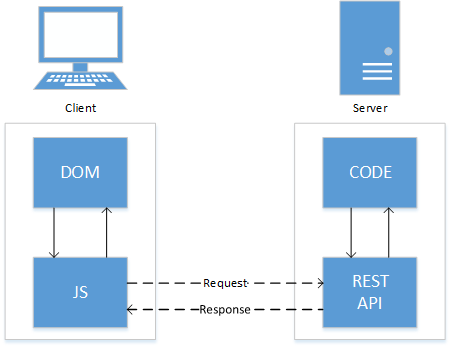
\includegraphics[width=0.6\textwidth, center]{StandDerTechnik/ClientServerJS}
    \caption[Client-Server Architektur mit Javascript]{Client-Server Architektur mit Javascript}
    \label{img:clientserverjs}
\end{figure}

In Abbildung \ref{img:clientserverjs} ist aufgezeigt, wie der Client mithilfe von Javascript mit
dem Server kommuniziert. Javascript holt
sich die Daten, die der Client benötigt und gibt diese dem DOM zum Verarbeiten weiter.

\subsection{Blazor WebAssembly}
Die Architektur von Blazor WebAssembly ist ähnlich zu den obig beschriebenen \ac{spa}s. Tatsächlich
verändert sich hierbei nur die Programmiersprache, die auf dem
Client läuft. Es handelt sich dabei um die Programmiersprache C\#, die auf dem Client
ausgeführt wird, wie im Folgenden zu sehen ist.
\begin{figure}[h]
    \centering
    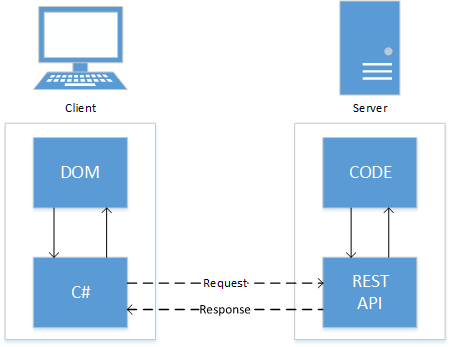
\includegraphics[width=0.6\textwidth, center]{StandDerTechnik/ClientServerCsharp}
    \caption[Blazor WebAssembly Architektur]{Blazor WebAssembly Architektur}
    \label{img:clientservercsharp}
\end{figure}
\newline
\newline
Das ganze Konzept C\# auf dem Client laufen lassen zu können, funktioniert durch
WebAssembly. WebAssembly wandelt Programmcode in nativen Bytecode um, der in einer Sandbox
im Browser ausgeführt werden kann. Dabei wird von der Sandbox aus die DOM mithilfe von
Javascript kontinuierlich manipuliert. Javascript verschwindet in dem Sinne also nicht komplett,
sondern wird lediglich ergänzt.
Da für dieses Konzept also WebAssembly vonnöten ist, kann Blazor WebAssembly nicht auf Browsern
funktionieren, die WebAssembly nicht unterstützen \cite{HierKommtBlazor}[vgl.].
\newline
\newline
Im Folgenden werden die Vor- und Nachteile von Blazor WebAssembly dargestellt:
\begin{itemize}
    \pro Sehr skalierbar
    \pro Sehr performant
    \pro Es kann komplett eigenständig auf dem Client laufen und ist nicht auf den
    Server angewiesen
    \con Große Anwendungsdatei, die auf dem Client geladen werden muss
    \con Lange Ladezeit beim ersten Aufruf
    \con Kompletter Code ist auf dem Client sichtbar
\end{itemize}

\subsection{Blazor Server}
Anders als bei Blazor WebAssembly der Fall ist, wird bei Blazor Server nicht C\# in den
Browser geladen, sondern der Code wird Serverseitig ausgeführt. Deswegen wird auch die
Web-Anwendung als SPA auf dem Server gerendert. Zum Client wird nur das JavaScript und Markup
gesendet. Die Daten und Benutzereingaben werden laufend mittels Signal R zwischen Client und Server
ausgetauscht. Dementsprechend ist es notwendig, dass immer zwischen dem Client und dem Server
eine offene Verbindung vorhanden ist \cite{HierKommtBlazor}[vgl.].
\newline
\newline
Dadurch das die komplette Seite auf dem Server gerendert wird, lädt die Seite auf dem Client sehr
schnell. Zudem muss lediglich eine kleine Javascript Datei auf den Client laden und die Seite
kann auf leistungsschwachen Clients verwendet werden.
\newline
\newline
Das ganze Konzept dieser Architektur baut drauf auf, dass beim ersten Aufruf der Seite eine
Javascript Datei names \emph{Blazor.js} auf dem Client geladen wird. Diese Datei kommuniziert
mit dem DOM und baut die Verbindung zum Server auf. Sobald die Verbindung aufgebaut ist, werden
kontinuierlich Nachrichten zwischen Client und Server ausgetauscht.

\begin{figure}[h]
    \centering
    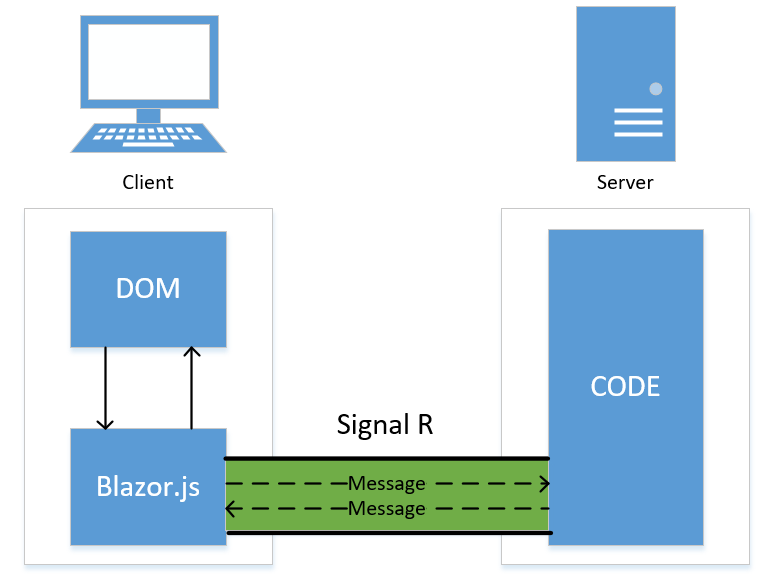
\includegraphics[width=0.6\textwidth, center]{StandDerTechnik/ClientServerSignalR}
    \caption[Serverarchitektur von Blazor]{Serverarchitektur von Blazor}
    \label{img:clientserversignalR}
\end{figure}

Im Folgenden werden die Vor- und Nachteile von Blazor Server zusammengestellt:
\begin{itemize}
    \pro Kurze Ladezeiten
    \pro Komplett browserunabhängig
    \pro Client hat keinen Zugriff auf den Sourcecode
    \pro Ist in der Lage mit leistungsschwachen Clients zu interagieren
    \con Nicht skalierbar, da alle Benutzer auf einem Server zugreifen
    \con Lange Netzwerklatenz führt zu Verzögerungen in der Benutzeroberfläche
    \con Es muss immer eine Verbindung bestehen
\end{itemize}